
\chapter{Didactic Manufacturing System}
\label{cha:system}
In this chapter, the system to be controlled and identified is presented.
The system is a didactic manufacturing system assembled from submodules fabricated
by Christiani\footnote{All images from the Christiani modules are present on its sales
  catalog, available at \url{www.christiani.de}. All rights are reserved to
  Christiani.}. This manufacturing system is located at the \LCA, located at the
\UFRJ.
% This
% system is normally used for the under-graduated studies about Industrial
% Automation and control of \DESs, and also for data acquisition in some
% bachelor\slash master\slash doctorate thesis, as this one.

The manufacturing system is a cube assembly system, where the different cube
halves shown in \autoref{fig:cubeHalves} are put together to form cubes.
\begin{figure}[H]
  \centering
  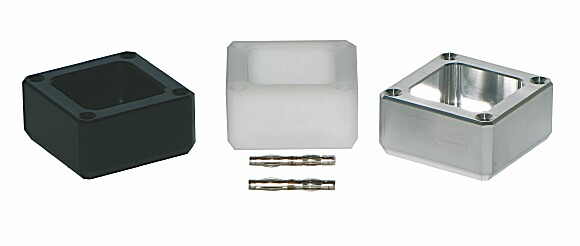
\includegraphics[width=0.55\textwidth]{maquete/pieces/workPieces.jpg}
  \caption{Cube halves.}
  \label{fig:cubeHalves}
\end{figure}

The pieces can be of two materials, metal or plastic, and the plastic ones can
be white or black.
The
permutation of cube halves needed to form a cube is selected via a type of
sorting, selecting the type of piece by material and colour. The assembled cubes
are then stored. In order to perform these tasks (sorting, handling, assembling
and storing), 6 Units are used. These units can be
seen in \autoref{fig:units}.

\begin{figure}[H]
\begin{subfigure}[t]{0.325\textwidth}
  \centering
  \includegraphics[width=\textwidth]{maquete/mag/mag.jpg}
  \caption{Magazine Unit}
\end{subfigure}
\hfill
\begin{subfigure}[t]{0.325\textwidth}
  \centering
  \includegraphics[width=\textwidth]{maquete/esteira/esteira.jpg}
  \caption{Conveyor Belt.}
\end{subfigure}

\begin{subfigure}[t]{0.325\textwidth}
  \centering
  \includegraphics[width=\textwidth]{maquete/sensores/sensores.jpg}
  \caption{Sorting Unit.}
\end{subfigure}
\hfill
\begin{subfigure}[t]{0.325\textwidth}
  \centering
  \includegraphics[width=\textwidth]{maquete/braco/braco.jpg}
  \caption{Handling Unit.}
\end{subfigure}

\begin{subfigure}[t]{0.325\textwidth}
  \centering
  \includegraphics[width=\textwidth]{maquete/prensa/prensa.jpg}
  \caption{Assembly Unit.}
\end{subfigure}
\hfill
\begin{subfigure}[t]{0.325\textwidth}
  \centering
  \includegraphics[width=\textwidth]{maquete/elevador/elevador.jpg}
  \caption{Storage Unit.}
\end{subfigure}
  \caption{Units of the Manufacture System.}
  \label{fig:units}
\end{figure}

In the next sections each unit and their Inputs\slash Outputs will be detailed.

\begin{observation}
What is described in the next sections as an input of a certain module, it is
considered as an output for the controller and vice versa.  
\end{observation}

\section{Magazine Unit}
\label{sec:magazine}
The magazine is a unit with the objective to store the cube halves to be used.
There are 2 types of magazines in the system, one to
 store pieces with connection pins inserted (the pins shown in
 \autoref{fig:cubeHalves}) and another to stock pieces without those pins. These
 magazine units
 can stack 8 and 10 pieces and will be denominated MAG 1 and MAG 2, respectively.
Each magazine has a pneumatic cylinder and a limit switch sensor. The cylinder serves to extract a
piece from the bottom of the stack, and the limit switch to know if the stack is empty
or not. Each one of these cylinders have 2 inputs that are used to extend and retract the cylinders (if they
are set to $true$). This kind of cylinder is called \emph{double acting
  pneumatic cylinder}. There are also 2
sensors used to know if the cylinders are extended or retracted, the output
is equal to $true$ if the respective condition is fulfilled. The inputs to
control the cylinders are called in this work \verb|Extend MAG 1/2 Cylinder| and
\verb|Retract MAG 1/2 Cylinder|, and the outputs are called \verb|MAG 1/2 Cylinder Extended| and
\verb|MAG 1/2 Cylinder Retracted|. The limit switch of each magazine outputs a $true$
value if the stack is empty and $false$, otherwise. Thus, the limit switches
are called in this work \verb|MAG 1/2 Empty|, and their localisation on the magazine
can be seen in \autoref{fig:magazine2}. 
\begin{figure}[H]
  \centering
  \begin{tikzpicture}
    \node[anchor=south west,inner sep=0] (image) at (0,0) {
      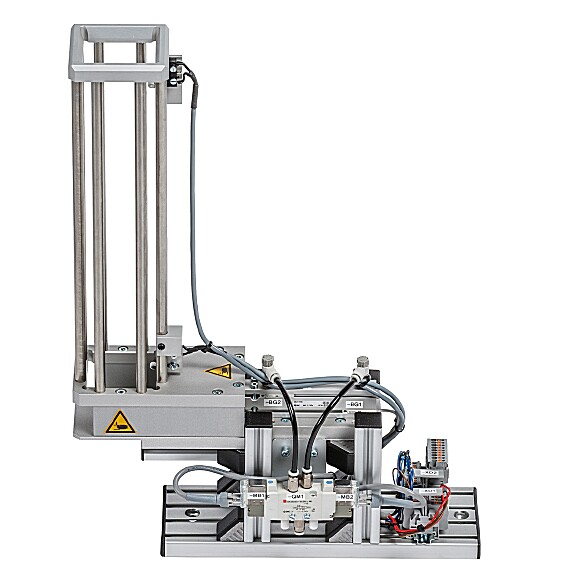
\includegraphics[width=8cm]{maquete/mag/30540_4.jpg}
    };
    % \draw[color1,ultra thick,rounded corners] (0,0) rectangle (9.4,6.2);
    \begin{scope}[x={(image.south east)},y={(image.north west)}]
        % \draw[help lines,xstep=.1,ystep=.1] (0,0) grid (1,1);
        % \foreach \x in {0,1,...,9} { \node [anchor=north] at (\x/10,0) {0.\x}; }
        % \foreach \y in {0,1,...,9} { \node [anchor=east] at (0,\y/10) {0.\y}; }
      \draw[color1] (0.85,0.55) node {\textbf{Cylinder}};
      \draw[<-,>=stealth,color1,very thick] (0.8,0.5) -- (0.67,0.37);
      \draw[color1] (0.75,0.7) node {\textbf{Limit switch}};
      \draw[color1,very thick, rounded corners] (0.25,0.35) rectangle (0.35,0.45);
      \draw[<-,>=stealth,color1,very thick] (0.6,0.65) -- (0.37,0.45);
      \end{scope}
  \end{tikzpicture}
  \caption{Magazine Unit.}
  \label{fig:magazine2}
\end{figure}

% only presence button
% \begin{figure}[H]
%   \centering
%   \begin{tikzpicture}
%     \node[anchor=south west,inner sep=0] (image) at (0,0) {
%       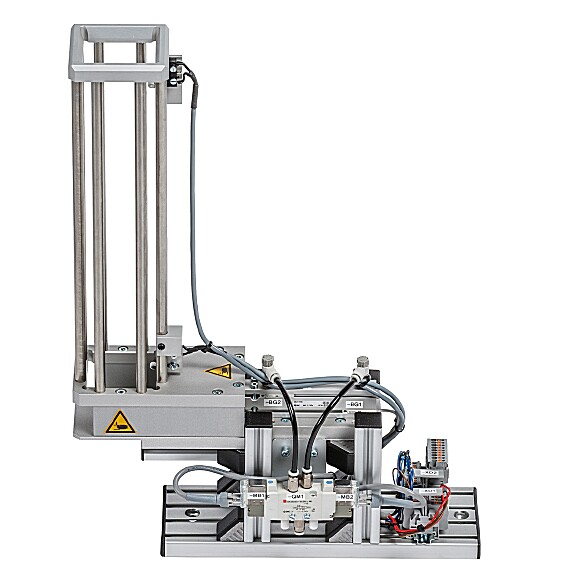
\includegraphics[width=8cm]{maquete/mag/30540_4.jpg}
%     };
%     % \draw[color1,ultra thick,rounded corners] (0,0) rectangle (9.4,6.2);
%     \begin{scope}[x={(image.south east)},y={(image.north west)}]
%         % \draw[help lines,xstep=.1,ystep=.1] (0,0) grid (1,1);
%         % \foreach \x in {0,1,...,9} { \node [anchor=north] at (\x/10,0) {0.\x}; }
%         % \foreach \y in {0,1,...,9} { \node [anchor=east] at (0,\y/10) {0.\y}; }
%       \draw[color1] (0.75,0.5) node {\textbf{Presence Button}};
%       \draw[color1,very thick, rounded corners] (0.25,0.35) rectangle (0.35,0.45);
%       \draw[->,color1,very thick] (0.5,0.5) -- (0.37,0.45);
%       \end{scope}
%   \end{tikzpicture}
%   \caption{Magazine Unit}
% \end{figure}

\section{Conveyor Belt}
\label{sec:magazine}
The conveyor belt transports the pieces from a
unit to another. It has 2 inputs and 1 output. The inputs are used to turn the
belt on, in two possible directions. The output is
generated by a presence sensor located at the end of the belt (see
\Autoref{fig:conveyorBelt}), and it is equal to $true$ if there is a piece in front
of it and $false$ otherwise. The directions of the movement of the pieces is
denominated Forward if it is going towards the presence sensor and Reverse if
not. Thus, the names given to the inputs that generate these movements are
\verb|Conveyor Belt Forward| and \verb|Conveyor Belt Reverse|.
The input is called \verb|Proximity Sensor End of Conveyor Belt|.

\begin{figure}[H]
  \centering
  \begin{tikzpicture}
    \node[anchor=south west,inner sep=0] (image) at (0,0) {
      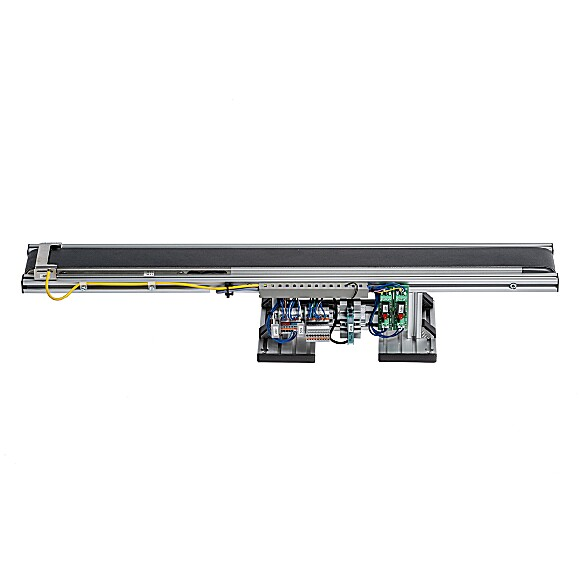
\includegraphics[trim={0 6cm 0 5cm},clip,width=8cm]{maquete/esteira/40778_3.jpg}
    };
    % \draw[color1,ultra thick,rounded corners] (0,0) rectangle (9.4,6.2);
    \begin{scope}[x={(image.south east)},y={(image.north west)}]
        % \draw[help lines,xstep=.1,ystep=.1] (0,0) grid (1,1);
        % \foreach \x in {0,1,...,9} { \node [anchor=north] at (\x/10,0) {0.\x}; }
        % \foreach \y in {0,1,...,9} { \node [anchor=east] at (0,\y/10) {0.\y}; }
        \draw [->,>=stealth,color1, very thick](0.9,0.75) -- ++ (-0.8,0.0);
        \draw [color1] (0.5,0.85) node {Forward};
        \draw [->,>=stealth,color1, very thick](0.1,0.95) -- ++ (0.8,0.0);
        \draw [color1](0.5,1.05) node {Reverse};
        
        \draw [color1](0.5,0.0) node {Presence Sensor};
        \draw [color1,very thick,rounded corners](0.05,0.45) rectangle (0.12,0.65);
        \draw [->,>=stealth,color1, very thick](0.1,0.4) -- (0.3,0.1);
      \end{scope}
  \end{tikzpicture}
  \caption{Conveyor Belt.}
  \label{fig:conveyorBelt}
\end{figure}

% no sensor
% \begin{figure}[H]
%   \centering
%   \begin{tikzpicture}
%     \node[anchor=south west,inner sep=0] (image) at (0,0) {
%       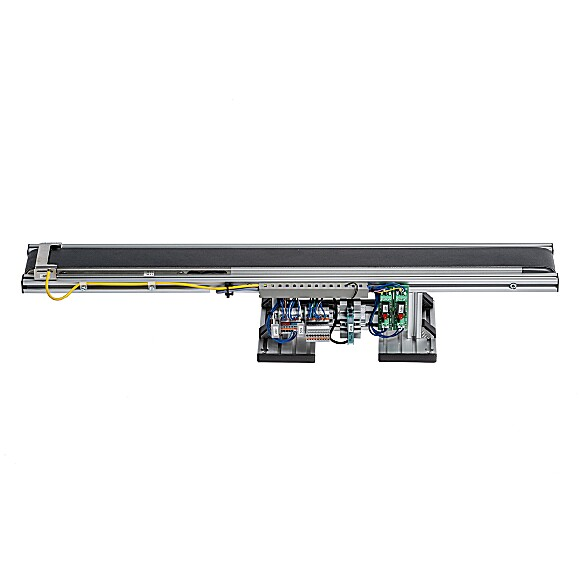
\includegraphics[trim={0 6cm 0 5cm},clip,width=8cm]{maquete/esteira/40778_3.jpg}
%     };
%     % \draw[color1,ultra thick,rounded corners] (0,0) rectangle (9.4,6.2);
%     \begin{scope}[x={(image.south east)},y={(image.north west)}]
%         % \draw[help lines,xstep=.1,ystep=.1] (0,0) grid (1,1);
%         % \foreach \x in {0,1,...,9} { \node [anchor=north] at (\x/10,0) {0.\x}; }
%         % \foreach \y in {0,1,...,9} { \node [anchor=east] at (0,\y/10) {0.\y}; }
%         \draw [->,>=stealth,color1, very thick](0.9,0.7) -- (0.1,0.7);
%         \draw [color1] (0.5,0.8) node {Forward};
%         \draw [->,>=stealth,color1, very thick](0.1,0.1) -- (0.9,0.1);
%         \draw [color1](0.5,0.0) node {Reverse};
%       \end{scope}
%   \end{tikzpicture}
%   \caption{Conveyor Belt}
% \end{figure}

\section{Sorting Unit}
\label{sec:sortingUnit}
The sorting unit is used to sort the pieces according to their material and colour.
In order to denominate its inputs and outputs, we will divide them in 2 parts,
identification and discharging.

The identification part uses 3 sensors to identify the type of the half cube: a
distance sensor to identify the orientation of the concavity of the piece, an
optic sensor to identify the colour of the plastic piece, and an inductive sensor
to identify the material of the piece. The output of the inductive sensor is
$true$ if the piece is made of metal, and $false$ if it is not, thus this output
is denoted as \verb|Metallic Sensor|. The output of the optic sensor is
equal to $true$ if the piece is reflexive (white) and $false$, otherwise
(black), thus it is denoted as \verb|White Color Sensor|. The distance sensor outputs
an integer value corresponding to the distance between the piece and the sensor, it is
denoted as \verb|Distance Sensor|, the logic used to find the orientation of the
piece is discussed in \Autoref{cha:control}.
The placement of these 3 sensors can be seen in \Autoref{fig:sortIden}. 
\begin{figure}[H]
  \centering
  \begin{tikzpicture}
    \node[anchor=south west,inner sep=0] (image) at (0,0) {
      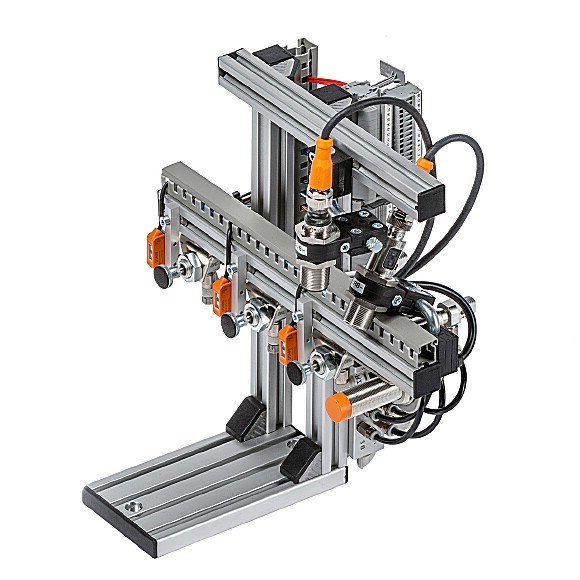
\includegraphics[trim={0 0 0 0},clip,width=8cm]{maquete/sensores/69511_2.jpg}
    };
    % \draw[color1,ultra thick,rounded corners] (0,0) rectangle (9.4,6.2);

    \begin{scope}[x={(image.south east)},y={(image.north west)}]
        % \draw[help lines,xstep=.1,ystep=.1] (0,0) grid (1,1);
        % \foreach \x in {0,1,...,9} { \node [anchor=north] at (\x/10,0) {0.\x}; }
        % \foreach \y in {0,1,...,9} { \node [anchor=east] at (0,\y/10) {0.\y};  }
        \draw[color1,ultra thick,rounded corners] (0.59,0.41) rectangle ++ (0.09,0.2);
        \draw[color1] (0.1,0.3) node {\textbf{Optic}};
        \draw[->,>=stealth,color1, very thick] (0.55,0.43) -- (0.2,0.32);
        \draw[color2,ultra thick,rounded corners] (0.48,0.47) rectangle ++ (0.09,0.3);
        \draw[color2] (0.1,0.8) node {\textbf{Distance}};
        \draw[->,>=stealth,color2, very thick] (0.45,0.6) -- (0.25,0.75);
        \draw[color3,ultra thick,rounded corners] (0.53,0.24) rectangle ++ (0.15,0.1);
        \draw[color3] (0.6,0.05) node {\textbf{Inductive}};
        \draw[->,>=stealth,color3, very thick] (0.6,0.2) -- (0.6,0.1);
      \end{scope}
  \end{tikzpicture}
  \caption{Sorting Unit - Identification.}
  \label{fig:sortIden}
\end{figure}

The discharging part is formed by 3 groups of inputs and outputs, denoted \emph{Left}, \emph{Center} and
\emph{Right}, as shown in \Autoref{fig:sortDisc}. 
Each group has a pneumatic cylinder and a presence sensor, and uses them to discharge pieces
depending on the logic of sorting and the identified piece by the identification
part of the sorting unit.
\begin{figure}[H]
  \centering
  \begin{tikzpicture}
    \node[anchor=south west,inner sep=0] (image) at (0,0) {
      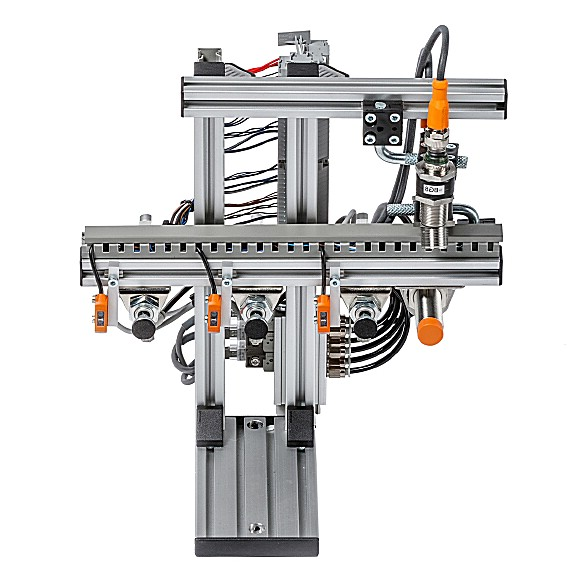
\includegraphics[trim={0 0 0 0},clip,width=8cm]{maquete/sensores/69511_3.jpg}
    };
    % \draw[color1,ultra thick,rounded corners] (0,0) rectangle (9.4,6.2);

    \begin{scope}[x={(image.south east)},y={(image.north west)}]
        % \draw[help lines,xstep=.1,ystep=.1] (0,0) grid (1,1);
        % \foreach \x in {0,1,...,9} { \node [anchor=north] at (\x/10,0) {0.\x}; }
        % \foreach \y in {0,1,...,9} { \node [anchor=east] at (0,\y/10) {0.\y};  }
        \draw[color1,ultra thick,rounded corners] (0.15,0.4) rectangle ++ (0.15,0.1);
        \draw[color1] (0.1,0.1) node {\textbf{Left}};
        \draw[->,>=stealth,color1, very thick] (0.2,0.38) -- (0.1,0.15);
        \draw[color2,ultra thick,rounded corners] (0.35,0.4) rectangle ++ (0.15,0.1);
        \draw[color2] (0.1,0.8) node {\textbf{Center}};
        \draw[->,>=stealth,color2, very thick] (0.4,0.52) -- (0.2,0.75);
        \draw[color3,ultra thick,rounded corners] (0.53,0.4) rectangle ++ (0.15,0.1);
        \draw[color3] (0.7,0.1) node {\textbf{Right}};
        \draw[->,>=stealth,color3, very thick] (0.65,0.38) -- (0.7,0.15);
      \end{scope}
  \end{tikzpicture}
  \caption{Sorting Unit - Discharging.}
  \label{fig:sortDisc}
\end{figure}
Differently from MAG 1/2, each cylinder is a \emph{single acting pneumatic cylinder}. When the corresponding input is equal to $true$ it
extends, and when it is $false$ it is automatically retracted.
A tag for each input is given depending on the group name, for
instance, to extend the left cylinder we use
\verb|Extend Left Discharge Cylinder| as input.
Each one of these cylinders has 2 outputs to determine if the cylinder is
extended or retracted, similarly the tags depend on the group, e.g.:
\verb|Right Discharge Cylinder Extended| and
\verb|Right Discharge Cylinder Retracted|.
The presence sensor of each group detects if there is a piece in front of the
cylinder, and its tag also depends on the group, e.g.:
\verb|Proximity Sensor Center Discharge Cylinder|.

\section{Handling Unit}
\label{sec:handlingUnit}
The handling unit is a robotic manipulator that serves to transfer the pieces
and eventually assembled pieces, from a unit to another. By the definitions of
robotic manipulators shown in \cite{khalil2004modeling}, this manipulator has 3
\DOF{}, and it is from the type called \emph{RPP}, as
it is formed by a Revolute joint and two Prismatic joints. The latter joints
being orthogonal regarding each other.

Since the position of its
\emph{end-effector} (the end of the robotic arm) can be described using a
cylindrical coordinate system, this kind of manipulator is also called
\emph{cylindrical shoulder}. With the end of easing the understanding of the
verbs used in this work to describe the movements of the manipulator, in this
section we will use beside these verbs the cylindrical coordinate
system ($\rho,\phi,z$), where $\rho$ is the axial distance, $\phi$ is the azimuth
and $z$ is the height.
The \emph{end-effector} of this manipulator is equipped with a vacuum suction
device capable of holding the pieces, which is controlled by an input called
\verb|Turn Vacuum Gripper On| that evidently turns the vacuum on when activated.

In order to control the position of the \emph{end-effector} of the manipulator, called
``arm'' throughout this work, there is a couple of pneumatic cylinders. The
behaviour of these cylinders is similar
to the behaviour of the cylinders in the sorting unit (\emph{single acting
  pneumatic cylinder}). These cylinders are placed in each
prismatic joint of the arm, thus raising (increasing the height $z$) and extending (increasing the
axial distance $\rho$) the arm when they are activated, respectively. The
respective inputs
of these cylinders are called \verb|Raise Arm| and \verb|Extend Arm|. Each
cylinder also has 2 sensors to identify if the are retracted or extended, and tags are given in the most mnemonic way possible, they are called
\verb|Arm Lowered|, \verb|Arm Raised|, \verb|Arm Retracted| and
\verb|Arm Extended|.

In order to rotate the revolute joint, a motor is placed
on the arm's base. This motor has two inputs that when activated makes the arm
rotate in one direction or the other, which will be called \CW{} and \CCW, and
the inputs that generate these kinds of movements denoted
\verb|Turn Arm CW| and \verb|Turn Arm CCW|.
In order to identify what is considered
\CW{} and \CCW{} it is needed to impose one of those rotation directions. In this
work we have imposed the \CCW{} direction as shown by the black arrow superposed to
the arm in \Autoref{fig:handlingUnit}. This same direction is considered as the
positive direction where the azimuth $\phi$ increases. The
\emph{zero position} of the arm azimuth ($\phi=0,$), is considered when the
\emph{end-effector} is diametrically opposed to the calibration pin shown in
\Autoref{fig:handlingUnit}. This pin as the name suggests is used for the
calibration of the arm. The arm has an inductive sensor in the opposite to the
\emph{end-effector} that is activated when
it is aligned to this pin.  The azimuth of the arm in \Autoref{fig:handlingUnit} is
$\phi=180^o$.

An encoder is used to measure the
azimuth angle, but as the angular velocity of the arm is relatively high, and
the resolution of the arm is very precise, the output of this encoder is connected to a High Speed
Counter, in order to correctly estimate the angle. The configuration
of the High Speed Counter can be seen in \cite{rochapereira2019automacao,antunesfloriano2019sincronizacao}.
\begin{figure}[H]
  \centering
  \begin{tikzpicture}
    \node[anchor=south west,inner sep=0] (image) at (0,0) {
      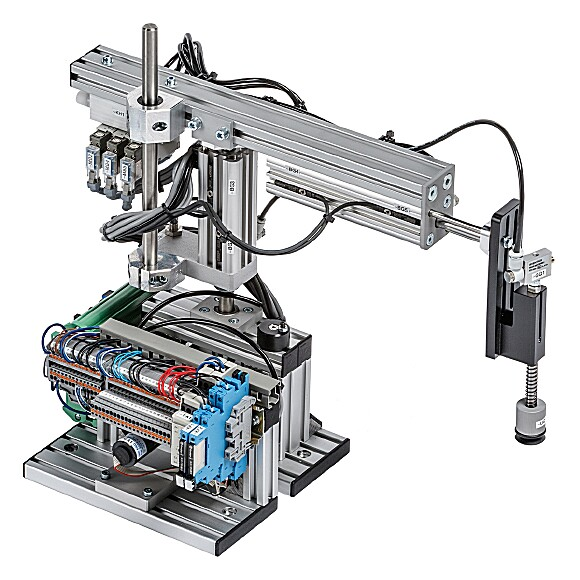
\includegraphics[trim={0 0 0 0},clip,width=8cm]{maquete/braco/69518_6.jpg}
    };
    % \draw[color1,ultra thick,rounded corners] (0,0) rectangle (9.4,6.2);

    \begin{scope}[x={(image.south east)},y={(image.north west)}]
        % \draw[help lines,xstep=.1,ystep=.1] (0,0) grid (1,1);
        % \foreach \x in {0,1,...,9} { \node [anchor=north] at (\x/10,0) {0.\x}; }
        % \foreach \y in {0,1,...,9} { \node [anchor=east] at (0,\y/10) {0.\y};  }
        % \draw [fill,white,fill opacity=0.4,draw=none] (0.1,0.8) rectangle  (0.4,0.96);
        \draw [color1,rounded corners, very thick] (0.43,0.4) rectangle  (0.5,0.45);
        \draw [->,>=stealth,color1, very thick] (0.51,0.384) -- (0.7,0.1);
        \draw [color1] (0.7,0.04) node {\textbf{Calibration Pin}};
        \begin{scope}[color1, scale=0.1]
          \draw[black, thick] (3.5,10) arc (0:180:1 and 0.3);
        \end{scope}
        \draw[->,>=stealth,color1, very thick] (0.255,0.8) -- (0.255,1.07);
        \begin{scope}[color1, scale=0.1]
          \draw[black,->,>=stealth,thick] (1.5,10) arc (180:350:1 and 0.3);
        \end{scope}
      \end{scope}
  \end{tikzpicture}
  \caption{Handling Unit.}
  \label{fig:handlingUnit}
\end{figure}

\newpage
\section{Assembly Unit}
\label{sec:assemblyUnit}
The assembly unit presses two pieces, resulting in a fully assembled
cube. As a safety measure, the assembly unit has a compartment made of
acrylic, in which a pneumatic cylinder is vertically arranged pointing downwards
to work as a press.
When the cylinder is extended, this press is lowered exerting a considerable
pressure on the pieces binding them together.
The inputs to lower and raise the press are called \verb|Lower Press| and
\verb|Raise Press|.

In order to open and close the compartment, there is an acrylic door combined
with a smaller pneumatic cylinder. When this cylinder is extended, the door
closes and when it is retracted the door opens. The inputs to open and close the
door are called \verb|Open Safety Door| and
\verb|Close Safety Door|. There are a couple of sensors to verify if the door is
opened or closed based on the extension and retraction of the cylinder, and their
respective outputs are called \verb|Safety Door Opened| and
\verb|Safety Door Closed|.

Since there is a safety compartment, where the cubes are assembled, there exists
a device with the purpose of transporting the pieces from outside to inside of
the press
and vice-versa. This device is called in this work
\verb|Assembly Unit Holder|, and as the name says it holds the pieces. This
device is coupled with another pneumatic cylinder that when it is retracted
it transports the \verb|Assembly Unit Holder| to the inner part of the
compartment, and outside the compartment if it is extended. The inputs that move
the \verb|Assembly Unit Holder| are called
\verb|Extend Assembly Unit Holder| and
\verb|Retract Assembly Unit Holder|. The outputs that indicate the extension and
retraction are called \verb|Assembly Unit Holder Extended|
and \verb|Assembly Unit Holder Retracted|. The position of the cylinders can be
seen in \Autoref{fig:assemblyUnit}.
\begin{figure}[H]
  \centering
  \begin{tikzpicture}
    \node[anchor=south west,inner sep=0] (image) at (0,0) {
      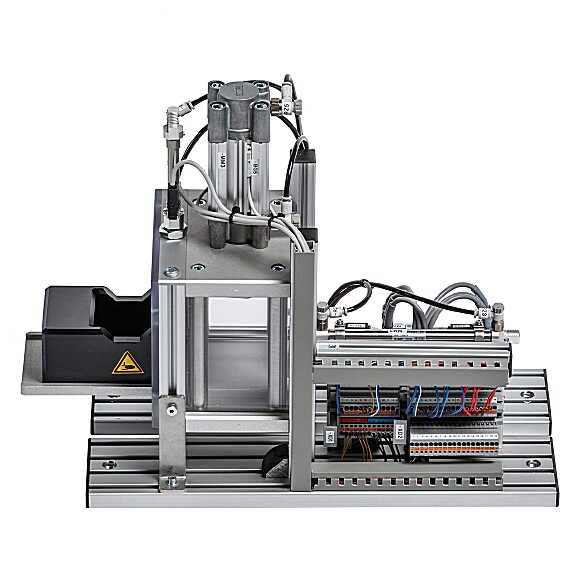
\includegraphics[width=8cm]{maquete/prensa/69514_4.jpg}
    };
    % \draw[color1,ultra thick,rounded corners] (0,0) rectangle (9.4,6.2);
    \begin{scope}[x={(image.south east)},y={(image.north west)}]
        % \draw[help lines,xstep=.1,ystep=.1] (0,0) grid (1,1);
        % \foreach \x in {0,1,...,9} { \node [anchor=north] at (\x/10,0) {0.\x}; }
        % \foreach \y in {0,1,...,9} { \node [anchor=east] at (0,\y/10) {0.\y}; }


        \draw[color2] (-0.1,0.8) node {\textbf{Door's Cylinder}};
      \draw[->,>=stealth,color2, very thick] (0.25,0.7) -- (0.1,.75);
      \draw[color2,ultra thick,rounded corners] (0.27,0.6) rectangle (.32,0.81);

      \draw[color3] (1,0.8) node {\textbf{Press' Cylinder}};
        \draw[->,>=stealth,color3, very thick] (0.5,0.8) -- (0.75,.8);
      \draw[color3,ultra thick,rounded corners] (0.34,0.57) rectangle (.47,0.87);


        \draw[color1] (0.7,0) node {\textbf{Holder's Cylinder}};
        \draw[->,>=stealth,color1, very thick] (0.7,0.38) -- (0.7,0.05);
      \draw[color1,ultra thick,rounded corners] (0.52,0.4) rectangle (.89,0.44);
      % \draw[color1] (0,0.5) node {\textbf{Left}};
      % \draw[color1] (0.5,1) node {\textbf{Top}};
      % \draw[color1] (0.5,0) node {\textbf{Bottom}};
      \end{scope}
  \end{tikzpicture}
  \caption{Assembly Unit.}
  \label{fig:assemblyUnit}
\end{figure}

\section{Storage Unit}
\label{sec:storageUnit}

The storage unit is a storage and retrieval system, but in this work
will be called only storage unit, since it will be its sole use.
The storage unit is a rack composed by 4 shelves, each one of them with enough space to
store 7 pieces, resulting in a total of 28 storage spaces. In order to elevate the
pieces, a motor with a spiral shaft is used to raise and lower the device where
the piece is placed to be stored. This piece holder is also called as
\verb|Storage Device| and sometimes as \verb|Storage Unit|, so when a movement
is given to the \verb|Storage Unit|, that means that this holder is moved and not the
rack itself.
There is also another motor that moves the
\verb|Storage Unit|
horizontally from Right to Left and vice versa.
As a reference for the direction of the movements of the
\verb|Storage Unit| used in this work, 
\Autoref{fig:storageUnit} shows what is considered the Right, Left, Top and
Bottom of this unit.

\begin{figure}[H]
  \centering
  \begin{tikzpicture}
    \node[anchor=south west,inner sep=0] (image) at (0,0) {
      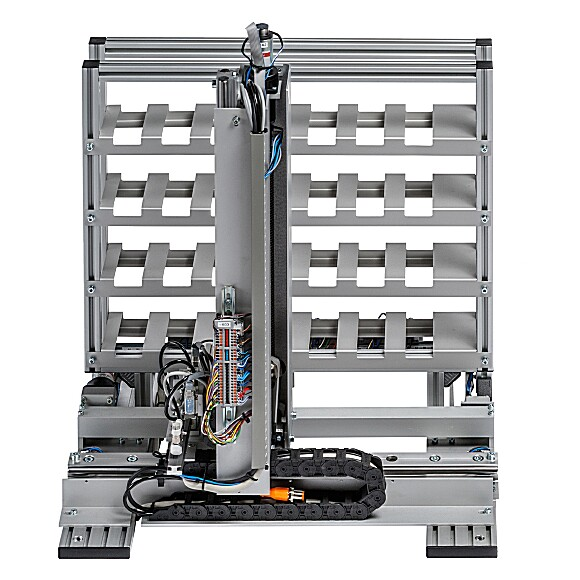
\includegraphics[width=8cm]{maquete/elevador/69523_3.jpg}
    };
    % \draw[color1,ultra thick,rounded corners] (0,0) rectangle (9.4,6.2);
    \begin{scope}[x={(image.south east)},y={(image.north west)}]
        % \draw[help lines,xstep=.1,ystep=.1] (0,0) grid (1,1);
        % \foreach \x in {0,1,...,9} { \node [anchor=north] at (\x/10,0) {0.\x}; }
        % \foreach \y in {0,1,...,9} { \node [anchor=east] at (0,\y/10) {0.\y}; }
      \draw[color1] (1,0.5) node {\textbf{Right}};
      \draw[color1] (0,0.5) node {\textbf{Left}};
      \draw[color1] (0.5,1) node {\textbf{Top}};
      \draw[color1] (0.5,0) node {\textbf{Bottom}};
      \end{scope}
  \end{tikzpicture}
  \caption{Storage Unit.}
  \label{fig:storageUnit}
\end{figure}
To effectively store the piece in the rack it is needed to move the
\verb|Storage Device| towards the rack. So, a pneumatic cylinder is coupled with
this device, and when the cylinder is extended, the device approaches the rack and
it leaves the rack when the cylinder is retracted. This cylinder is a
\emph{single acting pneumatic cylinder} and its input is called
\verb|Extend Storage Unit|. There are also 2 outputs to tell if the cylinder is
extended or retracted, called \verb|Storage Unit Extended| and
\verb|Storage Unit Retracted|.

The movement of the \verb|Storage Unit| is controlled by 4 inputs called \texttt{Move Storage Unit Upwards}, \texttt{Move Storage Unit Downwards}, 
\texttt{Move Storage Unit to the Right} and
\texttt{Move Storage Unit to the Left}.

In order to estimate the position of the \verb|Storage Device|  there are two
encoders, called \verb|Storage Unit Vertical Encoder| and
\verb|Storage Unit Horizontal Encoder|, that in conjunction with holes
specifically placed, aligned with the store spaces can identify if the device is
aligned with the store spaces. There are also 4 limit switches whose outputs
are called
\verb|Storage Unit Inferior Limit Switch|,
\verb|Storage Unit Superior Limit Switch|,
\verb|Storage Unit Right Limit Switch| and
\verb|Storage Unit Left Limit Switch| that have the purpose to indicate if the
\verb|Storage Device| is in one of the limits of the rack.


%%% Local Variables:
%%% mode: latex
%%% TeX-master: "../monografia"
%%% End:
